% ------ headers globales -------------
\documentclass[11pt, a4paper, twoside]{article}
\usepackage{header}
\usepackage{config}
% -------------------------------------
\begin{document}

% -- Carátula --
\clearpage{\pagestyle{empty}% parametros para la caratula (caratula.sty)

\materia{Sistemas Operativos}
%\submateria{}
\titulo{Trabajo Práctico 3}
\subtitulo{Algoritmos en sistemas distribuidos}
%\subtitulo{Escape en Sistemas}
\fecha{13 de noviembre de 2014}
\integrante{Rodriguez, Pedro}{197/12}{pedro3110.jim@gmail.com}
\integrante{Benegas, Gonzalo Segundo}{958/12}{gsbenegas@gmail.com}
\integrante{Barrios, Leandro Ezequiel}{404/11}{ezequiel.barrios@gmail.com}
%\grupo{Grupo ??}

\maketitle
\cleardoublepage}

%-- Índice --
\clearpage{%
  \pagestyle{empty}\tableofcontents%
  \vspace{3cm}%
  \begin{abstract}
  En el presente trabajo práctico estudiaremos algunos de los métodos más comúnmente utilizados 
  en la actualidad por distintos sistemas operativos para manejar correcta y eficientemente los 
  diversos procesos que se ejecutan concurrentemente en máquinas con uno o más procesadores.

  Intentaremos detectar las ventajas y desventajas de cada método, así como los escenarios en los
  cuales uno puede ser más eficiente que otro. Para esto, dividimos el TP en tres partes: en la
  primera, presentamos el simulador \texttt{simusched} y lo corremos para algunas tareas específicas. En la
  segunda parte, extendemos el simulador con nuevos schedulers implementados por nosotros y finalmente,
  en la tercera parte evaluamos y analizamos los distintos algoritmos de scheduling ya presentados.
  \end{abstract}
  \cleardoublepage%
}
%-- A partir de aquí, pongo el contador de páginas en 1 --
\setcounter{page}{1}

\index{Entendiendo el simulador simusched}
\section{Entendiendo el simulador simusched}

\subsection{Ejercicio 1}
En este ejercicio, programamos la tarea TaskConsola, que simularía una tarea interactiva con
el usuario. 

Para la implementación de esta tarea, primero tuvimos que registrarla para que el simulador la 
reconozca en el archivo \texttt{tasks.cpp}, con la función \texttt{tasksinit(void)}. En ese mismo archivo implementamos
la tarea, que para el proceso número $pid$ recibe los tres parámetros: $n$, $bmin$ y $bmax$. Simplemente
hacemos un ciclo que cicle n veces y que cada vez tome un entero al azar\footnote{para elegir 
el número pseudo-aleatorio hacemos uso de la función \texttt{rand()} provista
por la librerá standard de C.} $r$ entre $bmin$ y 
$bmax$, y cada vez llamamos a la función \texttt{usoIO(pid, r)}, que simula hacer uso de dispositivos de
entrada/salida. 

Se denomina llamada bloqueante a aquellas llamadas en las que, si lo que esta  
solicita no está disponible, entonces el proceso llamador se queda bloqueado a la espera de un
resultado. Es decir, no permite que otros procesos dependientes de éste sigan ejecutando. Por 
el contrario, en una llamada no bloqueante, si el proceso llamador no encuentra lo que estaba
buscando, el proceso devuelve de todas formas algún resultado, permitiendo que otros procesos
sigan ejecutando sin tener que esperar a que este proceso llamador reciba el resultado que está
esperando. 

\clearpage
\subsection{Ejercicio 2}
Para seguir entendiendo el funcionamiento del simulador simusched, ahora pasamos a escribir un lote
de 3 tareas distintas: una intensiva en CPU y las otras dos de tipo interactivo. Vamos a ejecutar y
graficar la simulación usando el algoritmo FCFS para 1, 2 y 3 núcleos. 

En el caso de la tarea que hace uso intensivo del cpu, pudimos observar que usando dos cpu's, las
tareas se logran ejecutar prácticamente en la mitad de tiempo (en el gráfico se ve claramente como
se aprovecha el hecho de que hay dos cpu's, y en todo momento se puede observar cómo hay dos cpu's 
trabajando al mismo tiempo en dos tareas distintas. Cuando introdujimos un tercer cpu, sucedió 
exactamente lo mismo: cada vez que algún cpu terminaba de ejecutar un proceso, inmediatamente
comenzaba a ejecutar el próximo proceso aún no atendido. 

En el caso de las tareas interactivas, pudimos observar los momentos en los que se detectaba que 
algún procesador era bloqueado y cómo en ese tiempo el procesador se quedaba trabado en la misma 
tarea. Creemos que ese tiempo de espera podría ser aprovechado para seguir ejecutando algún otro
proceso, implementando algún otro sistema de scheduling. 

Otra cosa importante a destacar, es que en los tres lotes de tareas, cuando pasamos de usar un único
core a usar dos, el tiempo total que se tardó en ejecutar todas las tareas disminuyó a la mitad.
Mientras que cuando usamos tres cores, el tiempo no disminuyó a un tercio de lo que tardaba antes,
que es lo que nosotros esperábamos. Esto nos da la pauta de que más procesadores no siempre
mucha más eficiencia y velocidad: hay otros factores que son más importantes, como el algoritmo de
scheduling utilizado, y la consideración de las características del lote de tareas que voy a querer
correr. 

A continuación, presentamos los diagramas de Gantt de los cuales hablamos: 

\begin{figure}[H]
  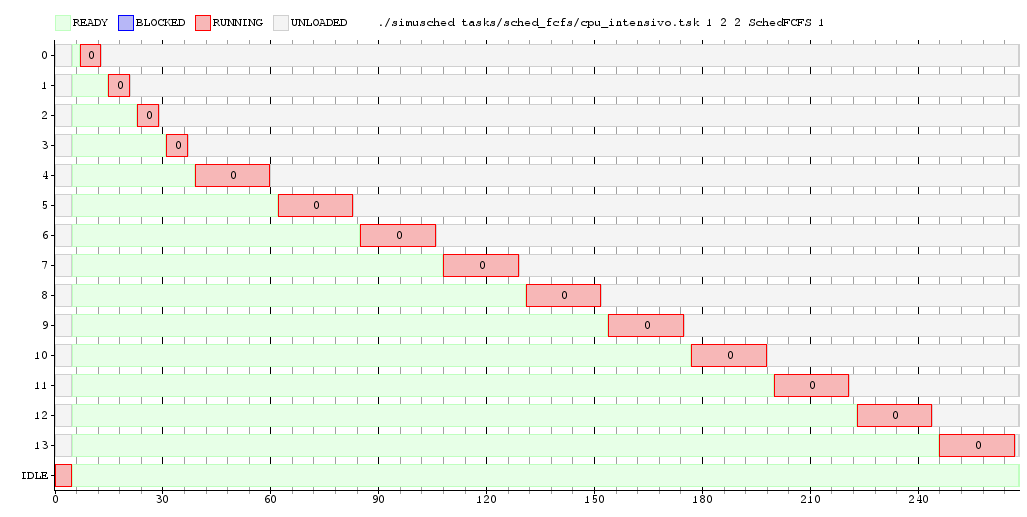
\includegraphics [width=\textwidth]{../graficos/sched_fcfs/cpu_intensivo.png}
  \caption{}
\end{figure}
\begin{figure}[H]
  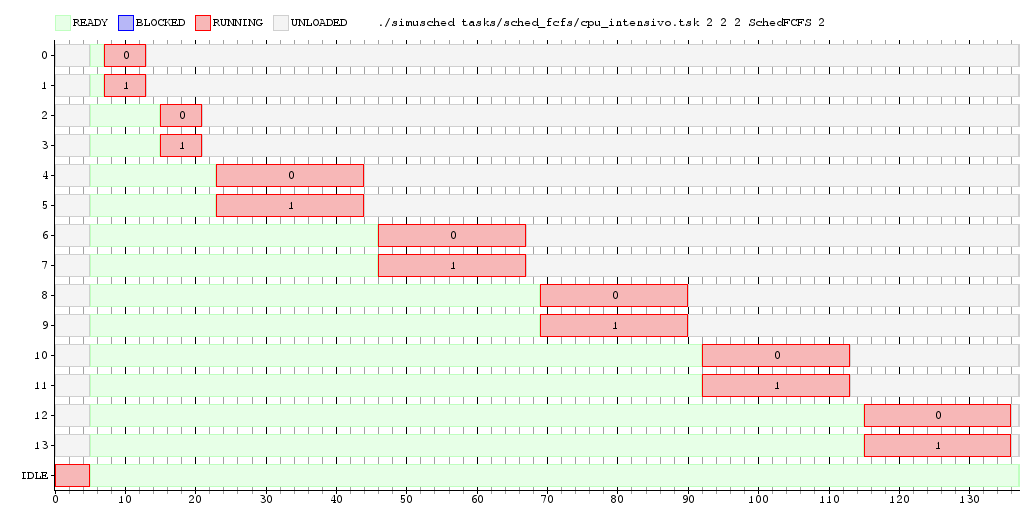
\includegraphics [width=\textwidth]{../graficos/sched_fcfs/cpu_intensivo2.png}
  \caption{}
\end{figure}
\begin{figure}[H]
  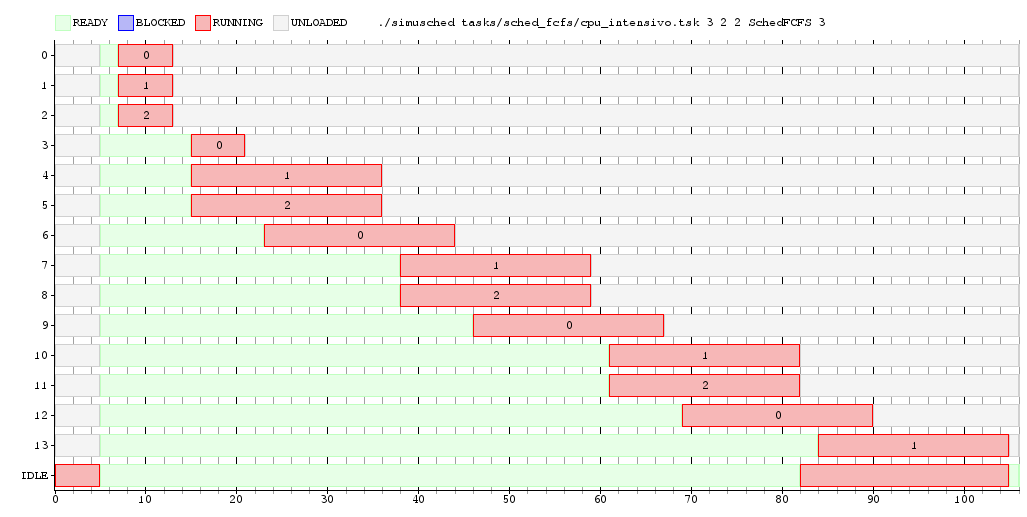
\includegraphics [width=\textwidth]{../graficos/sched_fcfs/cpu_intensivo3.png}
  \caption{}
\end{figure}
\begin{figure}[H]
  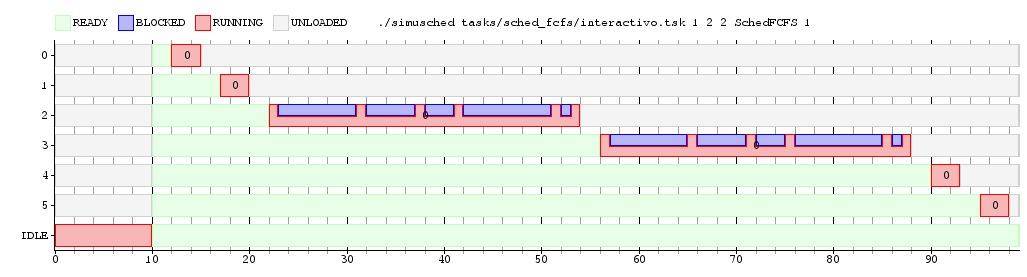
\includegraphics [width=\textwidth]{../graficos/sched_fcfs/interactivo.png}
  \caption{}
\end{figure}
\begin{figure}[H]
  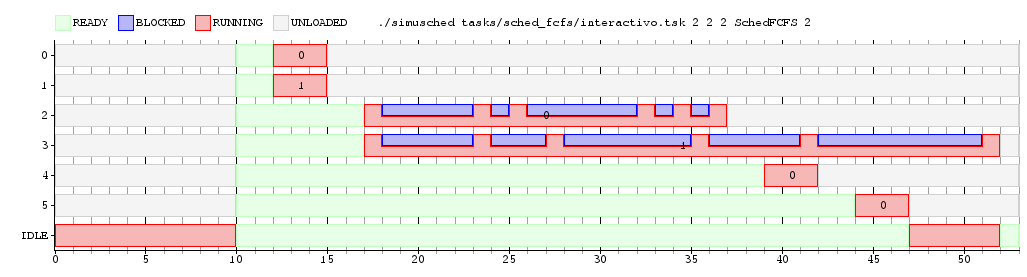
\includegraphics [width=\textwidth]{../graficos/sched_fcfs/interactivo_2.png}
  \caption{}
\end{figure}
\begin{figure}[H]
  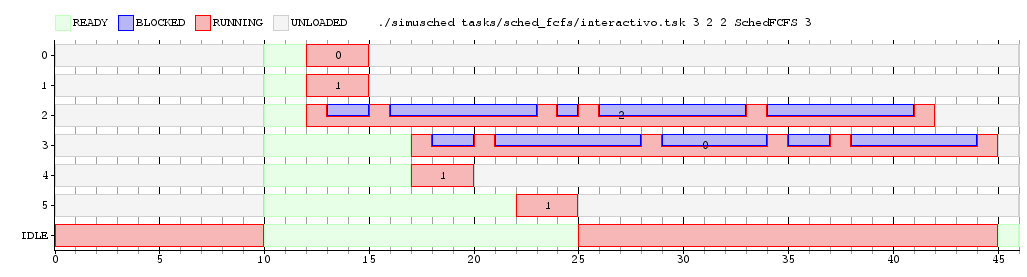
\includegraphics [width=\textwidth]{../graficos/sched_fcfs/interactivo_3.png}
  \caption{}
\end{figure}
\begin{figure}[H]
  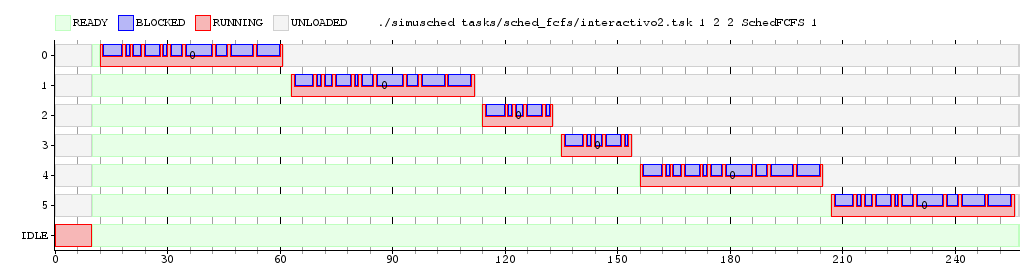
\includegraphics [width=\textwidth]{../graficos/sched_fcfs/interactivo2.png}
  \caption{}
\end{figure}
\begin{figure}[H]
  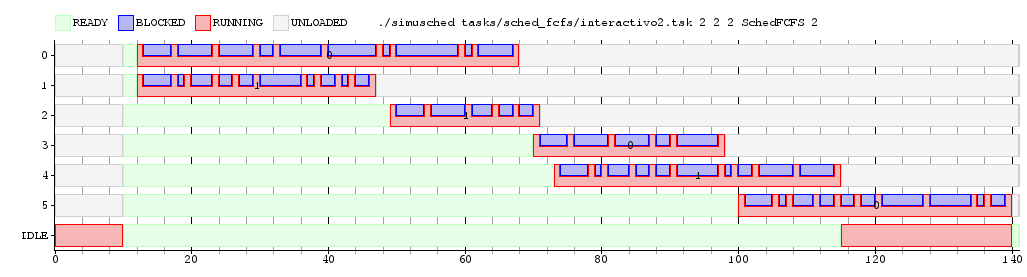
\includegraphics [width=\textwidth]{../graficos/sched_fcfs/interactivo2_2.png}
  \caption{}
\end{figure}
\begin{figure}[H]
  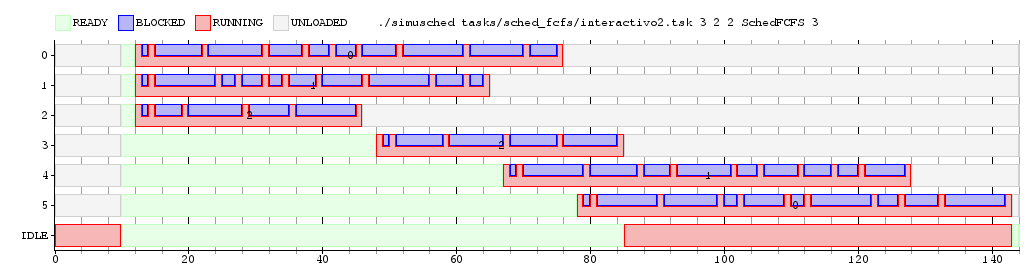
\includegraphics [width=\textwidth]{../graficos/sched_fcfs/interactivo2_3.png}
  \caption{}
\end{figure}

\clearpage





\index{Extendiendo el simulador con nuevos schedulers}
\section{Extendiendo el simulador con nuevos schedulers}
\setcounter{subsection}{2}

\subsection{Ejercicio 3}
Ahora pasaremos a explicar algunos aspectos relevantes de la implementación que hicimos del shceduler
$Round-Robin$, cuya idea básica es asignar espacios de tiempo equitativos a cada proceso y ir pasando
de uno a otro en forma circular, sin asignar ningún tipo de prioridad a ningún proceso. Una
característica interesante de este sistema de scheduling es que nos aseguramos de no tener el problema
conocido como $starvation$. 

En la implementación, recibimos como parámetro la cantidad de núcleos con la que vamos a trabajar
y los valores de sus respectivos $quantums$. Utilizamos una única cola global, para permitir así la
migración de proceso entre núcleos. La clase SchedRR consta de una parte pública y una privada. En 
la pública, se cuenta (al igual que en SchedLottery) con las funciones $load(pid)$, $unblock(pid)$ 
y $tick(cpu, motivo)$. La función de load es la de notificar al scheduler que un nuevo proceso ha llegado.
Cada vez que esto sucede, agregamos a la cola de procesos el pid del de dicho proceso. Unblock se encarga 
de que en la próxima llamada a la función tick, el proceso pid esté disponible para ejecutar. Y 
finalmente, tick se encarga de manejar, de acuerdo a qué fue lo último que hizo el proceso antes de llamar
a dicha función y a la porción del $quantum$ ya utilizado por el proceso, de encolar en la cola de procesos
al proceso actual y pasar a correr el próximo proceso si ya se utilizó todo el $quantum$, de pasar a correr 
el próximo proceso y dejar fuera de la lista de procesos al proceso actual si dicho proceso ha finalizado, o de
poner a correr el próximo proceso y encolar en la lista de procesos al proceso actual si dicho proceso se ha
bloqueado por alguna razón. 

Por otro lado, esta la parte privada de la clase SchedRR. Consta de algunas variables que utilizamos para efectuar
correctamente el manejo de procesos según la plítica del round-robin. Usamos un $vector<int> cores\_ticks$, 
con el que llevamos la cuenta en todo momento de la cantidad de ticks que consumió el proceso actual, 
para cada núcleo. También utilizamos un $vector<int> cores\_quantums$, en el cuál almacenamos los quantums
de cada procesador que nos son pasados por parámetro. Otra estructura de datos importante es una
$queue<int> process\_queue$, en la cuál almacenamos todos los procesos que están esperando a ser ejecutados.
En $cores_count$ guardamos la cantidad de núcleos con la que vamos a trabajar. Finalmente, implementamos la
función $run\_next(cpu)$, que devuelve el pid del próximo proceso de la cola a ejecutar. Sólo la invocamos
cuando es necesario pasar a ejecutar un nuevo proceso. Y lo que hacemos es sacar el primer proceso que está 
esperando en la cola de la misma y ponerlo a correr, al mismo tiempo que inicializamos la variable
$cant\_ticks[pid]$ a cero (inicializamos el contador de ticks para el proceso actual en ejecución a cero). 


\clearpage
\subsection{Ejercicio 4}

Para este ejercicio se pide diseñar lotes de tareas, y luego simularlos mediante el Scheduler
\texttt{SchedRR} implementado en el \textbf{punto 3}. Se diseñó un lote de tareas simples,

\begin{minipage}{5cm}
\begin{Verbatim}[frame=single,framesep=1cm,label=task\_sched\_rr.tsk]
*10 TaskCPU 5  
\end{Verbatim}
\end{minipage}

las cuales comienzan todas al mismo tiempo, y corren con los mismos parámetros, de forma tal que 
permiten visualizar rápidamente el comportamiento característico del \textbf{Round Robin}, tal y como
se puede apreciar en \fig{gantt-sched-rr}.

\begin{figure}[H]
  \centering
  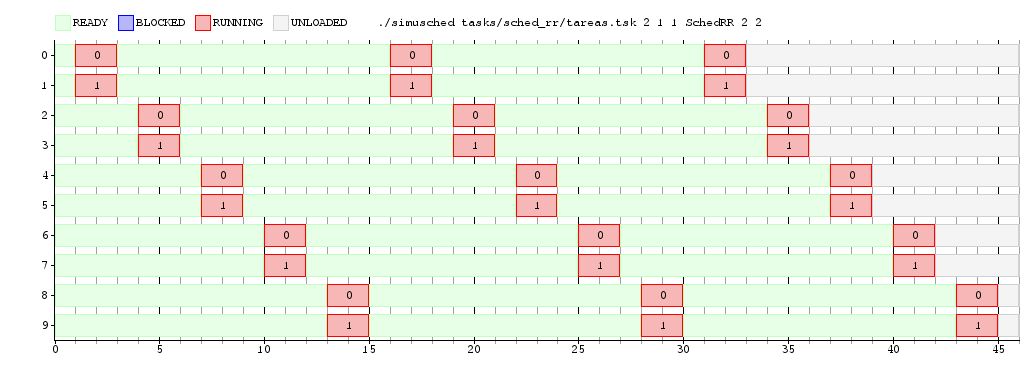
\includegraphics [width=\textwidth]{../graficos/sched_rr/output1.png}
  \caption{Diagrama Gantt de SchedRR}
  \label{fig:gantt-sched-rr}
\end{figure}

\clearpage
\subsection{Ejercicio 5}
En este ejercicio, basados en el paper de Waldspurger, C.A. y Weihl en el cuál presentan un 
novedoso sistema de Scheduling llamado $Lottery Scheduling$, implementamos una clase que llamamos
SchedLottery que recibe como parámetros el quantum que se va simular y una semilla 
pseudo-aleatoria, que el scheduler va a utilizar para el manejo de los procesos. Como dice en el
enunciado, básicamente nos interesó implementar la idea básica del algoritmo y la 
optimización de tickets compensatorios y en este caso, siempre trabajamos sólo con un núcleo. 

La clase SchedLottery tiene como parte pública las funciones \texttt{load(pid)}, \texttt{unblock(pid)} 
y \texttt{tick(cpu, motivo)}. 

i) La función load(pid) la utilizamos para notificar al scheduler
que un nuevo proceso ha llegado. Cada vez que llega un nuevo proceso le damos un ticket a dicho proceso.
De esta forma, en el próximo sorteo el proceso será candidato a ganarlo y así ser el próximo 
en ser ejecutado. 

ii) La función
tick(cpu, motivo). El parámetro motivo puede significar que una de tres cosas
ocurrieron durante el último ciclo del reloj: la tarea pid consumió todo su
ciclo utilizando el CPU número $cpu$ (en cuyo caso incrementamos la cantidad de ticks y si esta cantidad supera el
quantum de dicho procesador, la desalojamos), la tarea ejecutó una llamada bloqueante o permaneció 
bloqueada durante el último ciclo (en cuyo caso proveemos al proceso bloqueado la compensación 
de tickets correspondiente basándonos en el paper antes mencionado) ó porque la tarea pid 
terminó (en cuyo caso desalojamos la tarea
actual). Después de hacer estos chequeos, corremos \texttt{run\_lottery()} que se encarga de efectuar el 
sorteo de tickets para la próxima vez que se necesite elegir un proceso ganador y así asignarle 
los recursos necesarios. 

iii) La función unblock(pid) hace que en la próxima llamada a la función tick, el proceso pid 
esté disponible para ejecutar. Lo que hacemos, es entregarle al proceso pid la cantidad de tickets
que tenía el proceso antes de ser bloqueado multiplicado por la compensación correspondiente, que 
depende de qué fracción del quantum dicho proceso hizo del CPU. 

Por otro lado, la clase SchedLottery tiene una parte privada, que consta de variables como $quantum$, 
que usamos para saber el quantum que tiene disponible cada proceso para ejecutarse, $seed$, que
usamos como semilla para elegir el ticket ganador cada vez que hagamos un sorteo, $vector<ticket>$, que
usamos para saber qué tickets corresponden a cada proceso, $total\_tickets$ para tener rápido acceso
a la cantidad de tickets que hay distribuidos entre los procesos y $tick\_number$ que usamos para 
llevar la cuenta de cuántas veces llamamos a la función tick(cpu,motivo). Además, contamos con 
las funciones privadas $compensa(pid)$, $desaloja(pid)$ y $tickets\_index(pid)$. La primera se encarga de
calcular y asignar la compensación deseada a un proceso cuando corresponda; la segunda de que cuando
se bloquea un proceso, no esté disponible para ejecutar en la próxima ejecución de la función
tick(cpu,motivo). Es decir, que la probabilidad de ser elegible en el sorteo sobre los tickets sea cero.
Para eso, lo que hicimos fue sacarle todos los tickets temporalmente a dicho proceso. 


\clearpage
\index{Evaluando los algoritmos de scheduling}
\section{Evaluando los algoritmos de scheduling}
\setcounter{subsection}{5}

\subsection{Ejercicio 6}

Se registró un nuevo tipo de tarea, \texttt{TaskBatch(total\_cpu, cant\_bloqueos)}. Hace uso del CPU $total\_cpu$ ticks de reloj en total, entre los cuáles hace $cant\_bloqueos$ llamadas bloqueantes, distribuidas de manera uniforme y de duración un tick de reloj.
La implementación requirió elegir $cant\_bloqueos$ momentos entre 1 y $total\_cpu$. Para eso se guardó un arreglo de booleanos que mantiene que momentos ya fueron elegidos. Entonces se fueron generando momentos de manera pseudo\-aleatoria hasta elegir $cant\_bloqueos$ momentos \textit{distintos} para hacer llamadas bloqueantes. En el resto del tiempo, la tarea usa el procesador.

\clearpage
\subsection{Ejercicio 7}
\clearpage
\subsection{Ejercicio 8}
En esta sección implementamos una segunda versión para el scheduler tipo $Round-Robin$ que ya implementamos
en ejercicios anteriores. En este caso, el objetivo es no permitir la migración de procesos entre núcleos y
analizar qué sucede con la performance de este scheduler en comparación con el original para distintos lotes
de tareas. En principio, esperaríamos que en algunos tipos de lotes un algoritmo ande mejor que el otro
Esto es porque, por ejemplo, pensamos que si tenemos un 
único proceso que tarda mucho en completarse y no permitimos migración entre procesos, usando el método 
alternativo empeoraríamos la performance mientras que usando el otro método, el tiempo total que se tardaría
en finalizar el proceso se reduciría a la mitad. Sin embargo, si aparte de dicho proceso largo tuviéramos un
segundo proceso igual de largo, la implementación más eficiente sería la que no permite migración entre 
núcleos (así nos ahorraríamos de perder tiempo en cambios de contexto). Finalmente, en principio creemos que
si hubieran muchos más procesos que núcleos y de longitud similar, 
y no se permitiera la migración de procesos entre núcleos, los tiempos de finalización de distintos 
procesos serían muy dispares. Algo que, en principio es indeseable pues podría suceder que si a un proceso muy 
corto le toca justo el mismo core que a un proceso muy largo, este debería esperar mucho tiempo a que el largo
termine hasta que el procesador lo atienda. 

En nuestra implementación del la clase $SchedRR2$ para implementar las mismas tres funciones básicas que venimos
implementando en los anteriores schedulers (tick, unblock, load), utilizamos en la parte privada de la clase tres
estructuras para el manejo de los procesos: estas son un $vector<core>$, que contiene mucha de la información 
que teníamos en la implementación del $SchedRR$(en efecto, tenemos almacenado el quantum del core, la cantidad de
ticks actual, un vector de entero que lleva cuenta de los procesos activos en dicho core, una cola de esos procesos para
saber en qué orden ir ejecutándolos, y una función runNextProcess() que se encarga de sacar de la cola al
primer proceso y ponerlo a correr), pero en este caso efectuamos una distinción entre qué procesos están en cada
núcleo (antes, no nos importaba hacer esta distinción, porque como había migración de procesos entre 
núcleos, no nos importaba en qué núcleo estaba cada proceso). 

Hacemos uso de esta estructura a través de la función $getProcessCores(pid)$, que para 
el proceso pid nos devuelve un puntero al núcleo en el cuál está presente. Entonces, ahora
en cada tick del reloj de cada cpu, si el motivo es de bloqueo o terminación, entonces pasamos a correr en ese mismo
cpu al próximo proceso. Mientras que si llega un nuevo proceso, lo agregamos a la cola de procesos del cpu
en el cual se efectuó el tick y no en ninguno otro. 

\clearpage
\subsection{Ejercicio 9}

\begin{figure}[H]
\centering
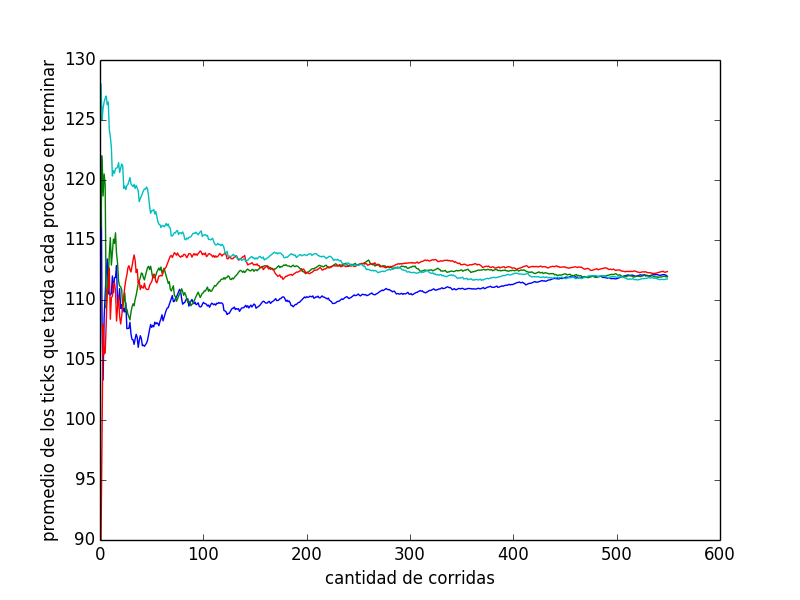
\includegraphics[scale=0.66]{../experimentacion/ej9-fairness/tiempo_final/prueba-tiempo-final.png}
\caption{Tiempo de ejecución de cuatro tareas idénticas}
\end{figure}

\begin{figure}[H]
\centering
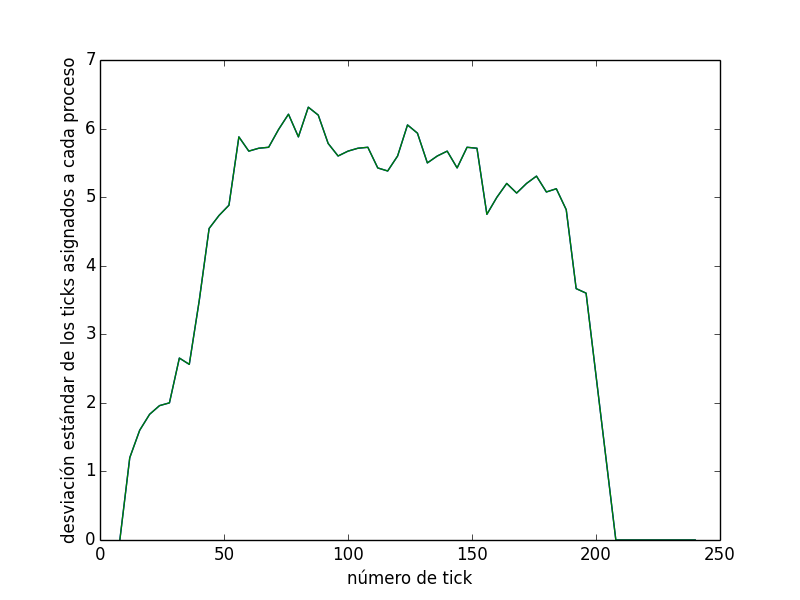
\includegraphics[scale=0.66]{../experimentacion/ej9-fairness/fairness/plot.png}
\caption{Desvío estándar de la cantidad de ticks asignados a cada proceso}
\end{figure}

\clearpage
\subsection{Ejercicio 10}

\begin{figure}[H]
\centering
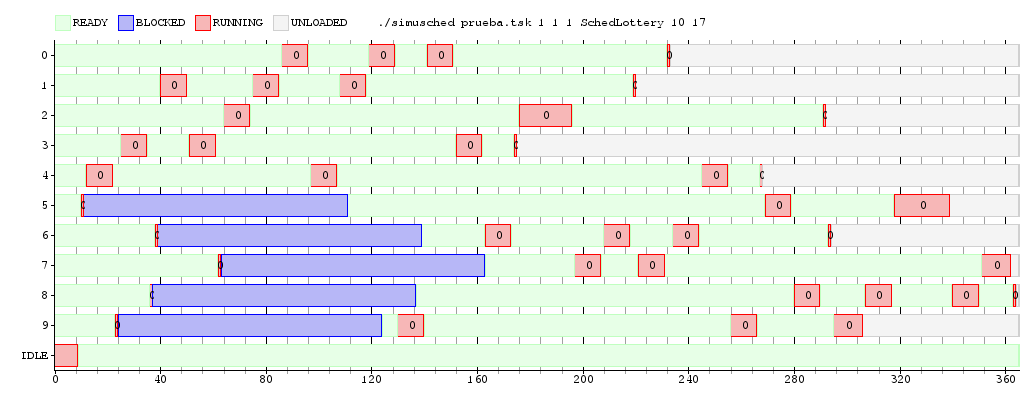
\includegraphics[scale=0.5]{../experimentacion/ej10-compensation/gant-sin.png}
\caption{Diagrama de $gant$ con $compensation\ tickets$}
\end{figure}

\begin{figure}[H]
\centering
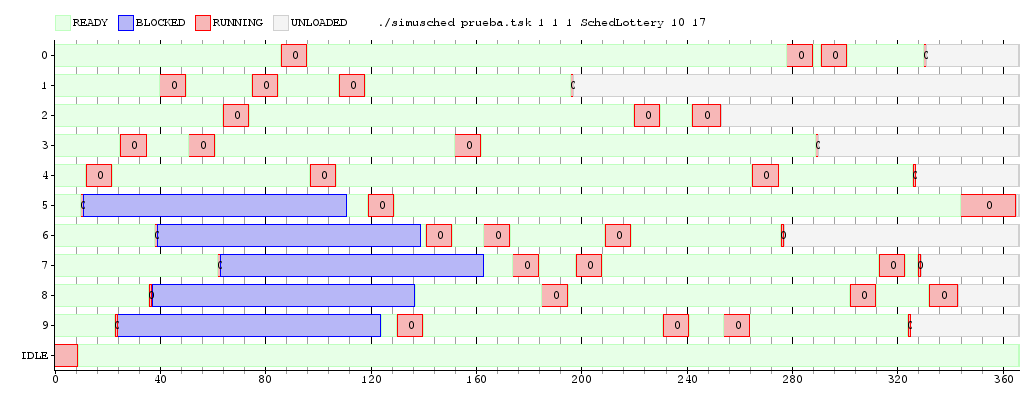
\includegraphics[scale=0.5]{../experimentacion/ej10-compensation/gant-con.png}
\caption{Diagrama de $gant$ sin $compensation\ tickets$}
\end{figure}

\begin{figure}[H]
\centering
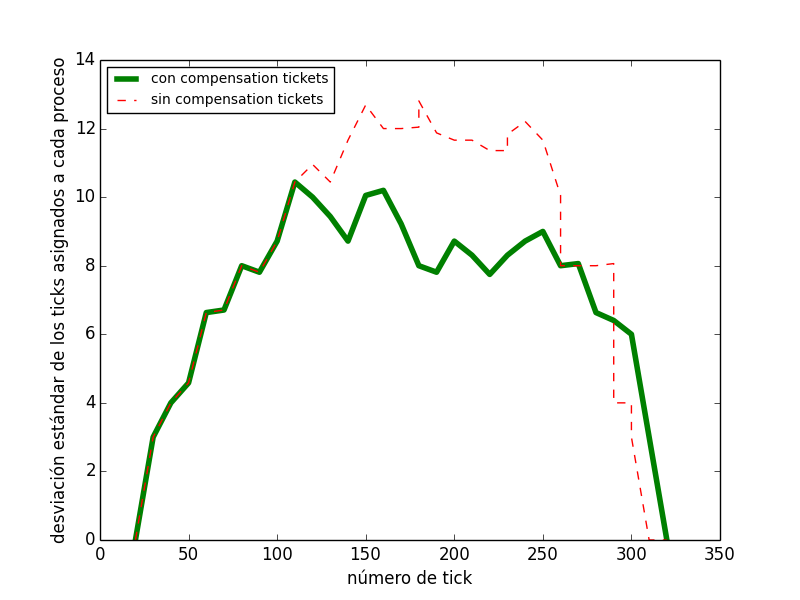
\includegraphics[scale=0.66]{../experimentacion/ej10-compensation/plot-comparativa.png}
\caption{Comparación de $fairness$ con y sin $compensation\ tickets$}
\end{figure}

\end{document}
